% !TEX root = ../main.tex

\chapter{The SBN program at Fermilab and the ICARUS experiment}
\label{chap:icarus_detector}

\section{The Short Baseline Neutrino program at Fermilab}
%% BRIEF INTRODUCTION
The Short Baseline Neutrino experimental program at Fermi National Accelerator Laboratories aims to  draw a complete and consistent picture of the sterile neutrino scenario, depicted in detail in \autoref{chap:theory_introduction}. 
% The main physics goal of the SBN collaboration is to test with great sensitivity the presence of a fourth sterile neutrino state, as suggested by multiple experimental anomalies. 
To achieve a level of statistical significance greater than $5\sigma$ for the LSND-allowed region (at \SI{90}{\percent} CL), SBN will carry out precision searches, recording millions of NC and CC neutrino interactions on argon. 

The key to such high sensitivity, other than the great statistic of events collected, is the design paradigm of the program. It will employ the Liquid Argon Time Projection Chamber (LArTPC) technology \cite{rubbiaLiquidArgonTime1977}, with two functionally identical detectors placed at different distances from the neutrino source. This way, the oscillatory behaviour is observed by comparing the neutrino flux at the far detector with the ``control'' flux recorded at the near detector, reducing the systematic uncertainties related to neutrino production and neutrino interaction in argon. 

Albeit the original plan for a three-detector program \cite{acciarriProposalThreeDetector2015}, MicroBooNE finished its data-taking period in 2020, two years prior to ICARUS starting its data collection campaign and five prior to SBND, so the SBN program will perform a search for the sterile neutrino as a two-detector experiment \cite{acciarriProposalThreeDetector2015, machadoShortBaselineNeutrinoProgram2019}. 

Both collect data from the common Booster Neutrino Beam (BNB); additionally, the ICARUS detector is located such that it is sensible to off-axis neutrinos coming from the Neutrino at the Main Injector (NuMI) beam. 

ICARUS is the far detector for the SBN programme, employing an active mass of \SI{476}{\tonne} of liquid argon (LAr), at a distance of \SI{600}{\meter} from the neutrino source; its position was chosen so as to maximise the oscillation probability. The ICARUS detector started its data taking independently from the SBN program in June of 2022, after the initial commissioning phase. It has now finished the fourth data collection campaign, collecting $\sim \SI{7.54e20}{POT}$ (proton-on-target), corresponding to about \num{e6} neutrino events.

At a distance of \SI{110}{\meter}, SBND is the near detector of the SBN program, with an active LAr mass of \SI{112}{\tonne}. After commissioning, it started data taking in December of 2024, joining the far detector and allowing for a precise knowledge of the neutrino flux. 

\paragraph{Oscillation measurements with a two-detector experiment} The main physics goal of the SBN program is the search for a fourth sterile neutrino state in the $3+1$ model. Using multiple LArTPC detectors, a high-sensitivity search for a high-$\Delta m^2$ splitting is possible by studying muon-neutrino oscillations in the $\PGnGm\to\PGnGm$ disappearance and $\PGnGm\to\PGne$ appearance channels. 

\begin{figure}
    \centering
    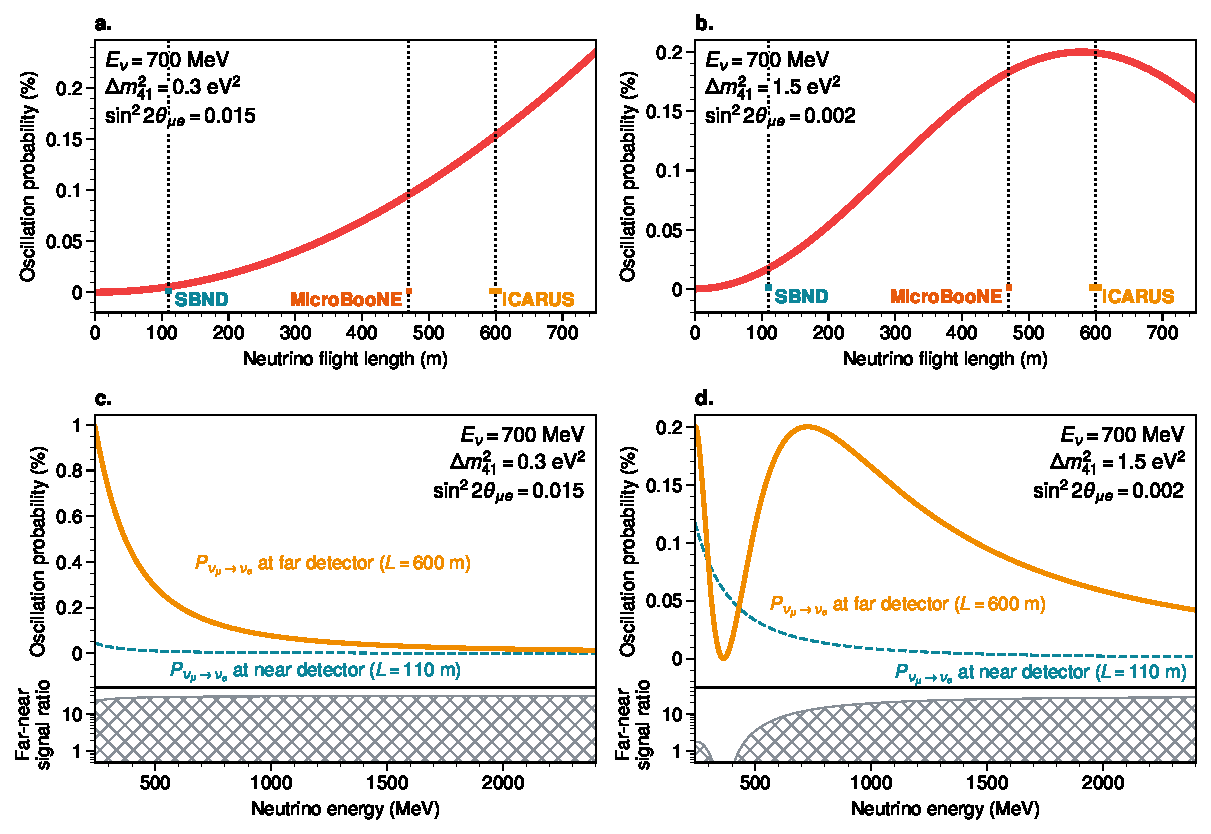
\includegraphics[width=\linewidth]{thesis/6_figures/SBN_sensitivity/appearance_signal.pdf}
    \caption[Electron neutrino appearance probability in the $3+1$ sterile oscillation scenario]{(a) and (b) show the oscillation probability for a \SI{700}{MeV} muon neutrino into an electron neutrino as a function of the length of the neutrino flight using two benchmark values of $(\sin^22\theta_{\PGm\Pe}, \Delta m^2)$. (c) and (d) show the same oscillation probability as a function of the neutrino energy. Additionally, the bottom panels show the far-over-near ratio. Adapted from \cite{machadoShortBaselineNeutrinoProgram2019}.}
    \label{fig:oscillation_2body_SBN}
\end{figure}

The oscillation probability for both channels is presented in \eqref{eq:2body_oscillation_sterile_disapp} and \eqref{eq:2body_oscillation_sterile_app} for the disappearance and appearance channels, respectively, with the assumption of the $3+1$ model. Looking at the $\PGnGm\to\PGne$ appearance channel, from the experimental results shown in \autoref{fig:all_experimental_searches}, the allowed parameter space lies in $\sin^22\theta_{\PGm\Pe} \in (\num{e-3},\num{e-1})$ and $\Delta m^2 \in (\num{e-1}, \num{e1})\ \si{eV^2}$; the location of the near and far detector  has been optimised to maximise the oscillation probability in this region of parameters. \autoref{fig:oscillation_2body_SBN} show $P(\PGnGm \rightarrow \PGne)$ for two benchmark values of $(\sin^22\theta_{\PGm\Pe}, \Delta m^2)$, assuming a neutrino energy of $\sim\SI{700}{MeV}$. Exploiting the strong correlations between the fluxes collected at the near and far detectors --- both use the same interaction medium and functionally identical revelation techniques --- the major impacting systematic uncertainties, which are those arising from the production mechanisms and the $\PGn$-Ar interaction cross-sections, can be mitigated in the two-detector configuration. 

With a planned collected statistics of \SI{6.6e20}{POT}, the $\PGnGm\to\PGnGm$ disappearance channel can also be probed to search for neutrino oscillation mediated by a sterile state. The unitarity of the $3+1$ PMNS matrix has to be preserved so that in the event of $\PGnGm\to\PGne$ appearance, meaning a nonzero value of $\sin^22\theta_{\PGm\Pe}$, a nonzero value of $\sin^22\theta_{\PGm\PGm}$, or a $\PGnGm\to\PGnGm$ disappearance signature, should be observed. 

Both channels will be studied to either pinpoint the correct $(\sin^22\theta, \Delta m^2)$ values or exclude some regions in the parameter space. \autoref{fig:sbn_2det} shows the projected excluded and allowed regions of the parameter space in both the \ref{sub@fig:nue_app_sbn_2det} $\PGne$-appearance and \ref{sub@fig:numu_disapp_sbn_2det} $\PGnGm$-disapperance channels of the two-detector operation of the SBN experiment. It should be noted that the projected \SI{6.6e20}{POT} was the original plan that was presented in the experiment proposal \cite{acciarriProposalThreeDetector2015}; however, BNB will operate until 2027, allowing the ICARUS detector to collect three times the statistics in standalone operation. 

\begin{figure}
    \centering
    \subfloat[]{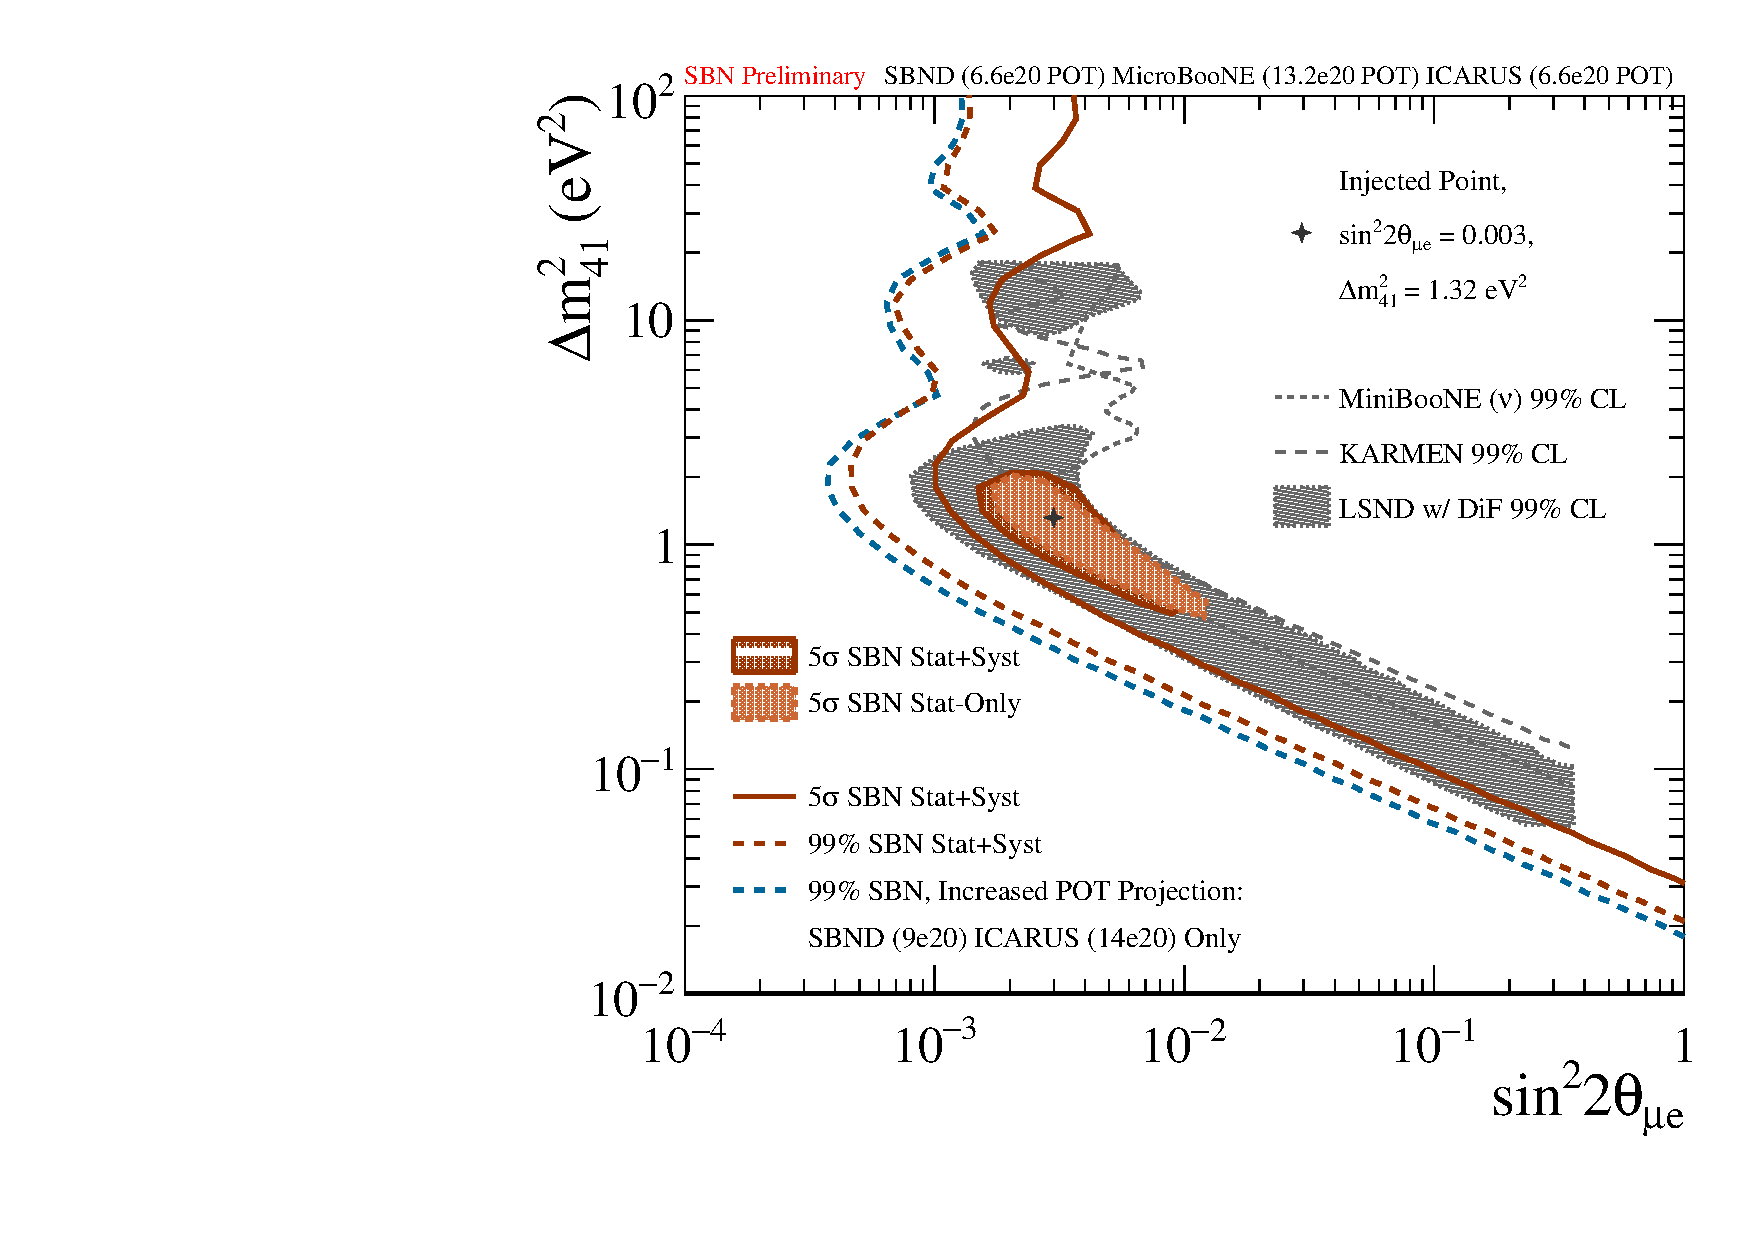
\includegraphics[width=0.5\linewidth]{thesis/6_figures/SBN_sensitivity/nue_app_2det_newPOT_sensitivity_comparison.pdf}\label{fig:nue_app_sbn_2det}}
    \subfloat[]{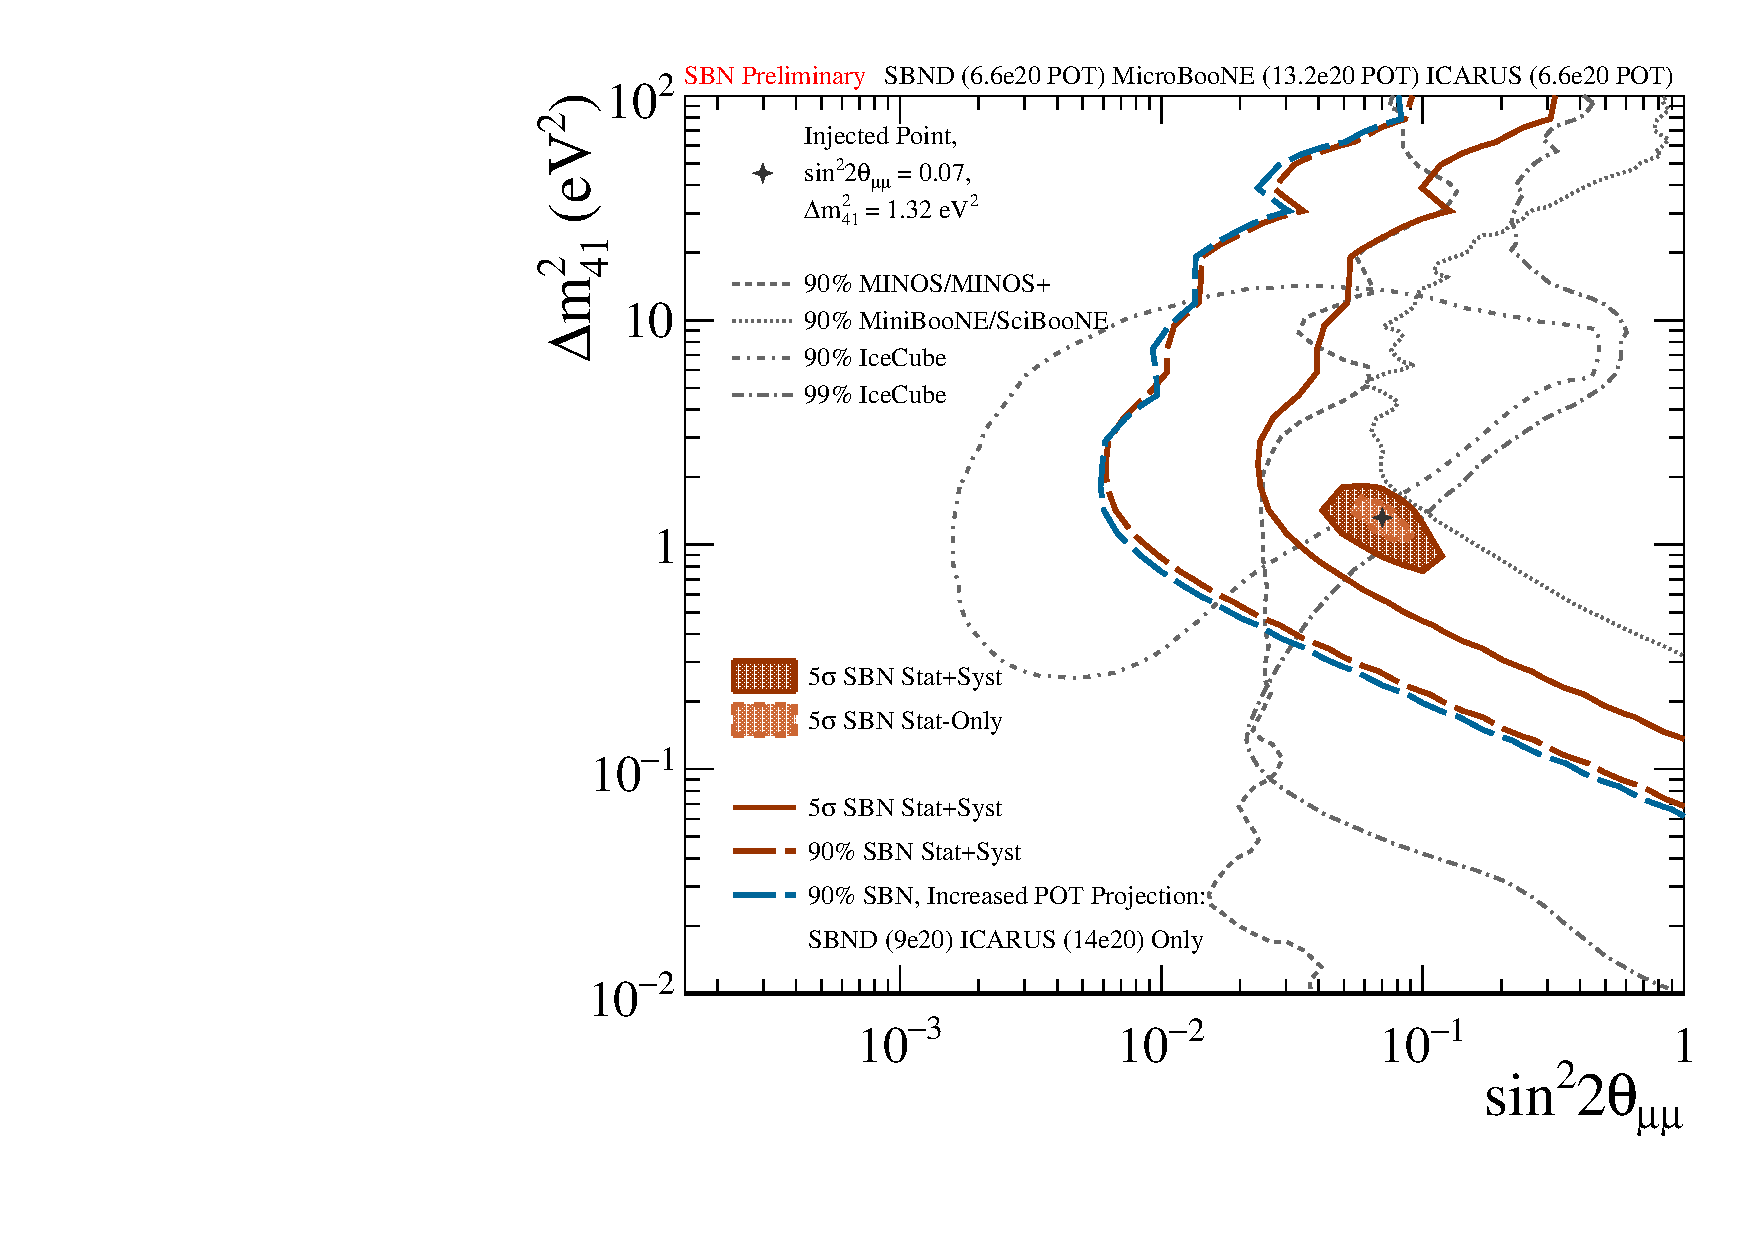
\includegraphics[width=0.5\linewidth]{thesis/6_figures/SBN_sensitivity/numu_disapp_2det_newPOT_sensitivity_comparison.pdf}\label{fig:numu_disapp_sbn_2det}}
    \caption[SBN sensitivity plots in both appearance and disappearance channels]{\ref{sub@fig:nue_app_sbn_2det} and \ref{sub@fig:numu_disapp_sbn_2det} show, respectively, the expected sensitivity curves in the $\PGne$-appearance and $\PGnGm$-disappearance channels under the hypothesis of no observation (solid and dashed lines, respectively at $5\sigma$ and 99\% CL) and under the hypothesis of observing an oscillatory signature in both channels (filled regions). These projections account for a collected \SI{6.6e20}{POT} and a two-detector configuration. }
    \label{fig:sbn_2det}
\end{figure}

Additionally, since a nonzero value of both $\sin^2 2\theta_{\PGm\Pe}$ and $\sin^22\theta_{\PGm\PGm}$ leads to a nonzero value of $\sin^22\theta_{\Pe\Pe}$, both the ICARUS detector, making use of the Booster and NuMI neutrino beams, and the SBND detector, only with data from the Booster beam, will explore the $\PGne$-disappearance channel $\PGne\to\PGne$. The combined result of this multi-channel search will provide strong evidence in favour of or against the $3+1$ sterile neutrino scenario. 

\paragraph{Cross-sections and BSM physics} In addition to the primary physics goals, the SBN programme, with its two LArTPC detectors, delivers a rich physics opportunity. 

Starting from particle interaction in liquid argon, both SBND and ICARUS detectors will use the Booster and NuMI (ICARUS-only) neutrino beams to perform cross-section measurements, exploiting the great amount of collected data with both detectors. 
For SBND, the proximity with respect to the neutrino source leads to a very large flux collected by the detector --- each run approximately of \SI{2.2e20}{POT} corresponds to 1.5M $\PGnGm$ and \num{12000} $\PGne$s; 
the same measurements can be performed with the ICARUS detector, which at the moment benefits from a longer data collection period and an accumulated statistic of \SI{7.5e20}{POT} in standalone operation. The larger dimension of the ICARUS detector also allows for more contained events, where all the final state interactions (FSI) are contained inside the detector active volume, allowing for a better particle identification (PID). 
Additionally, the position of the ICARUS detector allows the collection of neutrinos from the NuMI beam at an off-axis angle of \SI{6}{\degree} with respect to BNB direction. 
The added value of the NuMI beam comes from the energy range it covers. 
Using protons from the Main Injector at an energy of \SI{120}{GeV}, it is able to cover the \qtyrange{1}{3}{GeV} energy range, which overlaps greatly with the DUNE operational energy range. Neutrinos from the NuMI beam will also feature an enriched electronic component from the three-body decay of the kaon, allowing for precise $\PGne$ cross-section measurements. At the moment of writing this thesis, two $\PGnGm$ charged current mesonless cross-section analyses, $\PGnGm\mathrm{CCN>1}\Pp0\PGp$ and $\PGnGm\mathrm{CCN}\Pp0\PGp$, are being carried on and are in the final phases before publication. 

Finally, exploiting the great tracking and calorimetric power of liquid argon TPCs, with exceptional precision and high-performance event reconstruction capabilities, opens up invaluable opportunities for new physics searches. Using high-intensity neutrino beams, with large statistics, it is possible to explore beyond standard model theories. A detailed description of possible searches is presented in refs. \cite{machadoShortBaselineNeutrinoProgram2019, acciarriProposalThreeDetector2015}. 
Recently the first physics paper by the ICARUS collaboration was published, exploring some of these BSM models involving the scalar sector using data from the NuMI beam \cite{icaruscollaborationSearchHiddenSector2025}. 

\subsection{Neutrino beam}

The location for the SBN programme was selected to make use of the already existing accelerator infrastructure at Fermilab. \autoref{fig:accelerator_complex} shows the FNAL accelerator complex schematic overview. This complex provides a powerful beam of neutrinos using protons extracted from the Booster accelerator, core to the operation of the SBN experiment, as well as multiple other particle beams (neutrinos and muons, as well as protons) which are employed in other experiments, such as the Neutrinos at the Main Injector Beam. 

The common starting point is the Linac (linear accelerator), boosting protons up to \SI{400}{MeV} of energy (or $\sim\SI{954}{MeV}$ of momentum) using radiofrequency (RF) cavities. Accelerated protons are extracted and boosted to an energy of \SI{8}{GeV} within the Booster ring. 

\begin{figure}
    \centering
    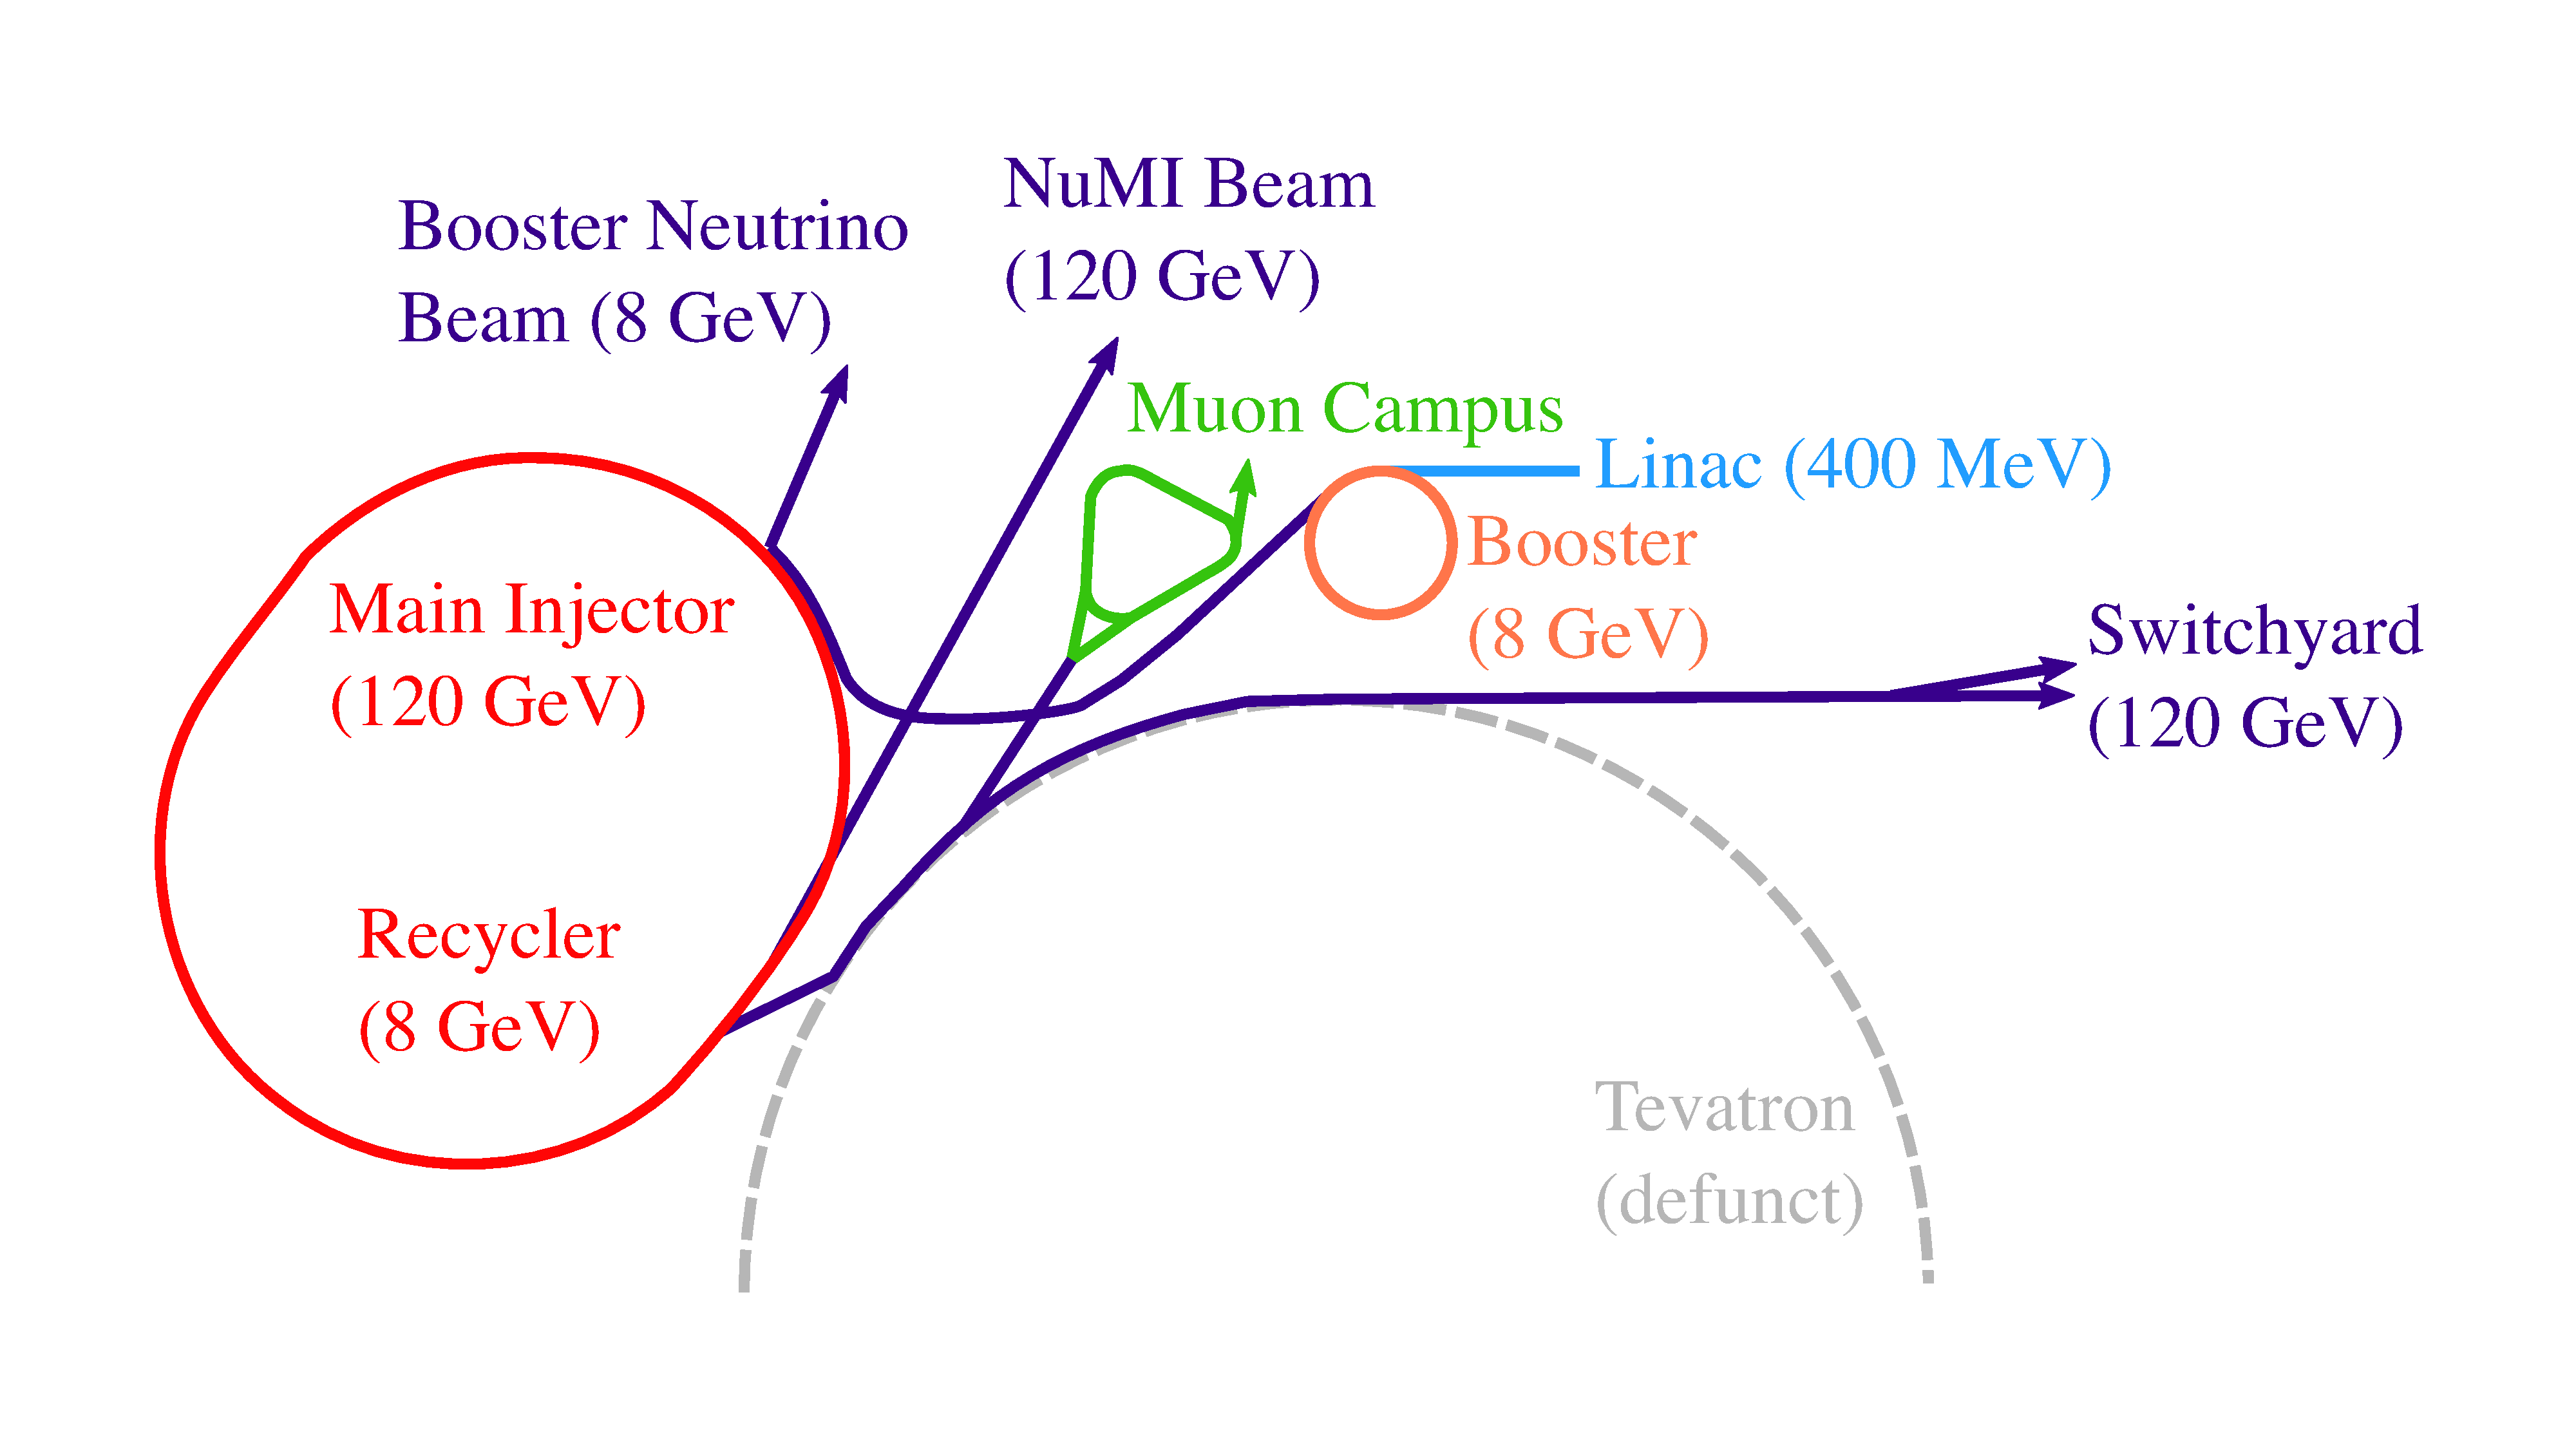
\includegraphics[width=0.75\linewidth]{thesis/6_figures/detector/BNB_NuMI_beams.pdf}
    \caption[Fermilab Accelerator complex]{Schematics of the accelerator complex at Fermilab. Both Booster and NuMI neutrino beams serve the ICARUS detector, with different energy  ranges, \SI{700}{MeV} for BNB and \SI{2.5}{GeV} for NuMI. Taken from \cite{ainsworthHighIntensityOperation2020}.}
    \label{fig:accelerator_complex}
\end{figure}

From the Booster ring, a fraction of protons is extracted to be used for the Booster Neutrino Beam, whereas the remaining fraction is sent into the Main Injector accelerator. From there a second Neutrino beam is extracted, the Neutrinos at the Main Injector (NuMI) beam. 

\begin{figure}
    \centering
    \subfloat[]{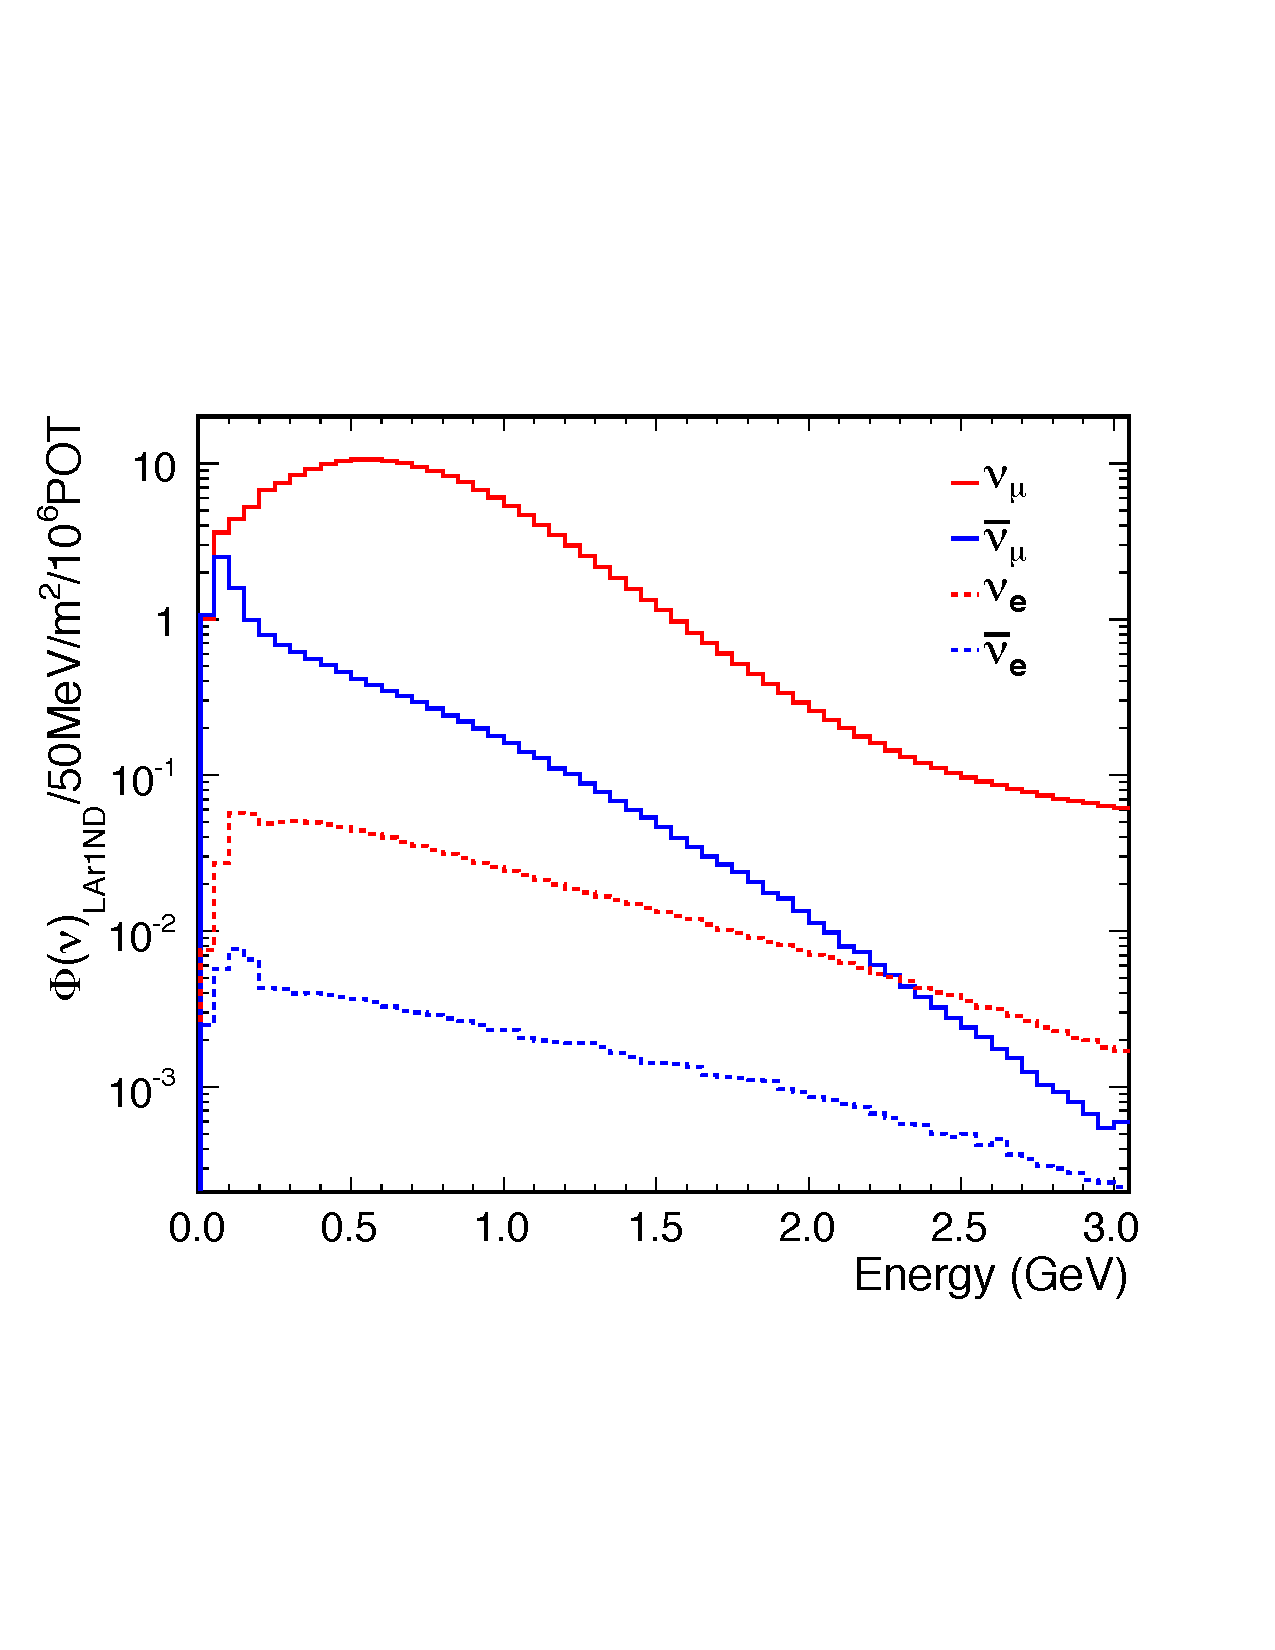
\includegraphics[trim={0 6cm 0 6cm}, width=0.5\linewidth]{thesis/6_figures/beams/BNB_flux_lar1nd.pdf}\label{fig:BNB_flux_SBND}}
    \subfloat[]{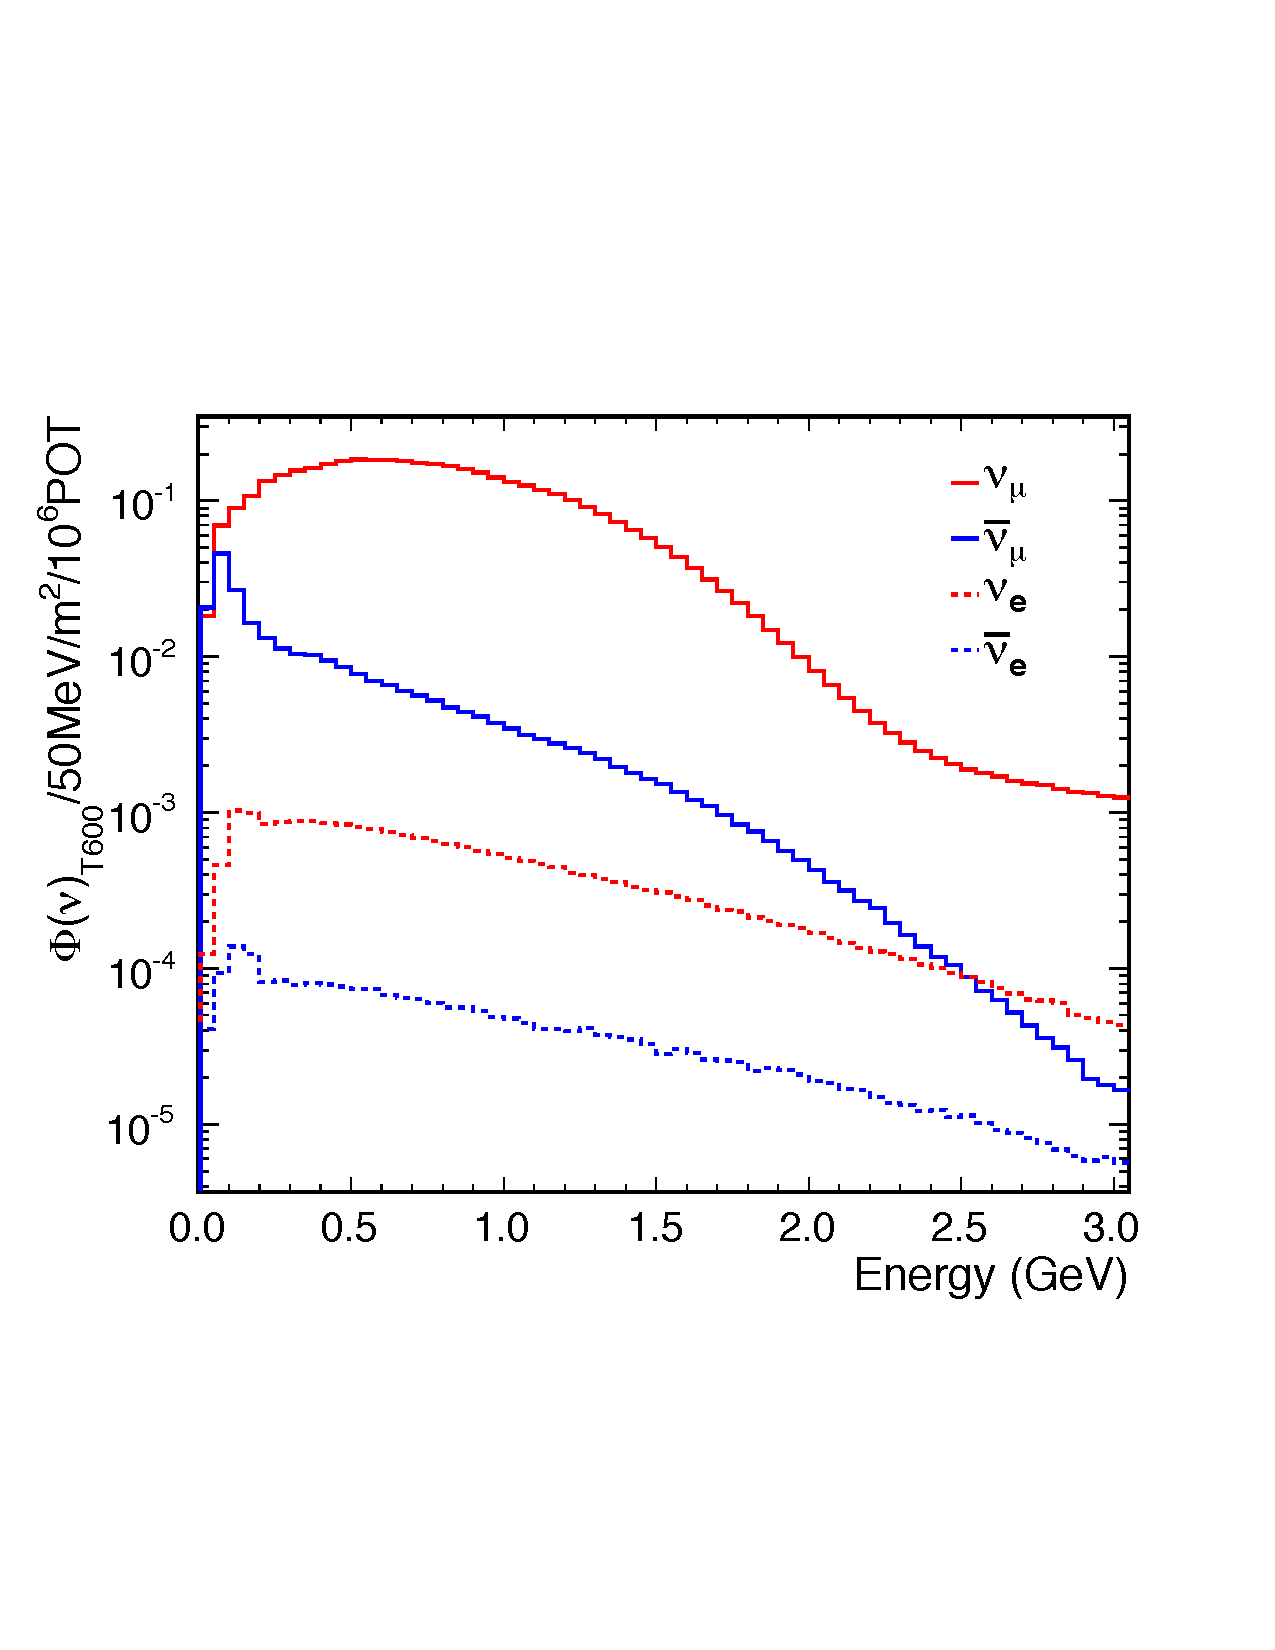
\includegraphics[trim={0 6cm 0 6cm}, width=0.5\linewidth]{thesis/6_figures/beams/BNB_flux_icarus.pdf}\label{fig:BNB_flux_ICARUS}}

    % \subfloat[]{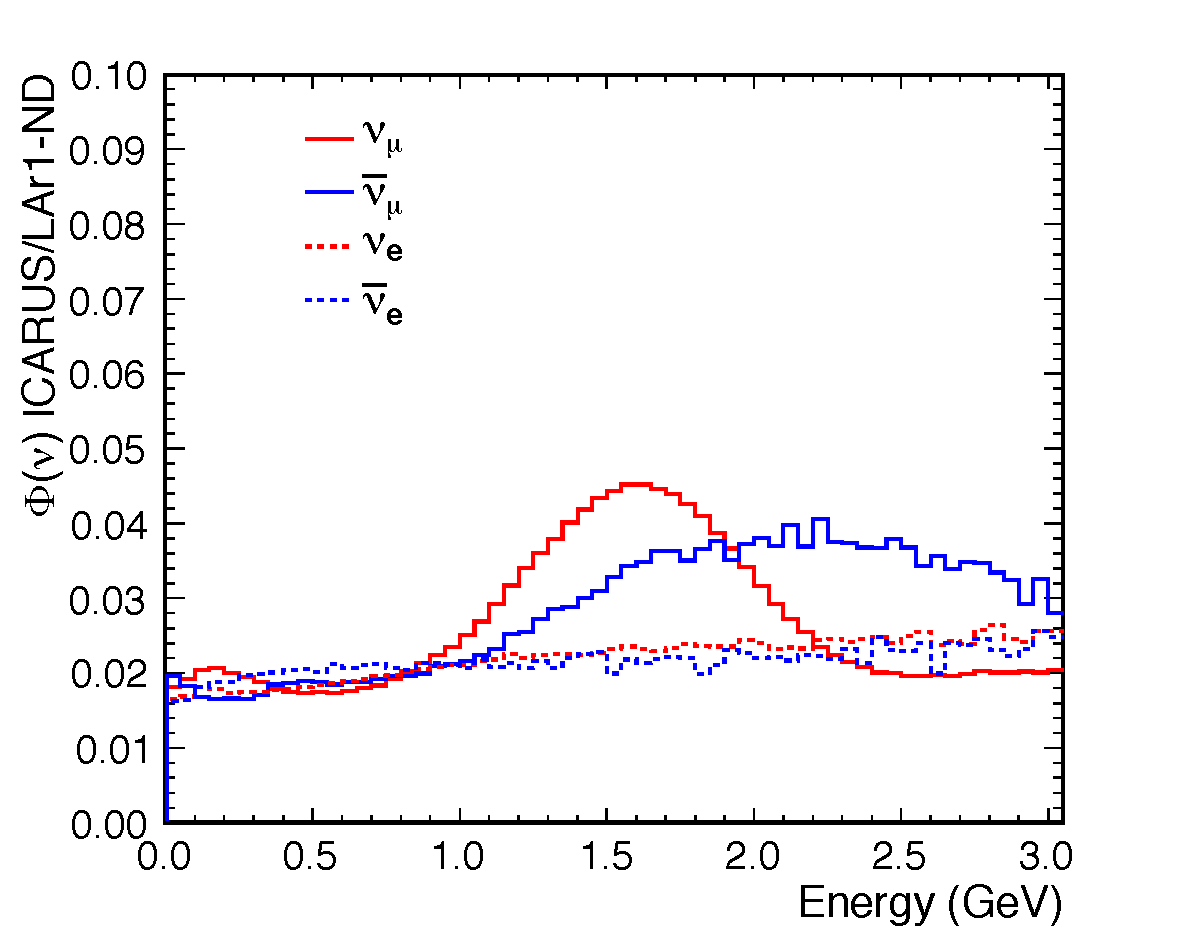
\includegraphics[trim={0 0cm 0 0cm}, width=0.5\linewidth]{thesis/6_figures/beams/BNB_flux_ratio_icarus_lar1nd.pdf}\label{fig:BNB_flux_ICARUS_SBND_ratio}}
    \caption[BNB flux predictions at the near and far detectors]{Predictions of the neutrino flux as computed by the MicroBooNE collaboration \cite{miniboonecollaborationNeutrinoFluxPrediction2009} at distances of \SI{110}{m} \ref{sub@fig:BNB_flux_SBND} and \SI{600}{m} \ref{sub@fig:BNB_flux_ICARUS} from the beryllium target, i.e., for the SBND and ICARUS detectors, respectively. }
    % \ref{sub@fig:BNB_flux_ICARUS_SBND_ratio} shows the predicted ratio of the two fluxes under the hypothesis of no sterile-mediated oscillation anomaly. }
    \label{fig:BNB_flux}
\end{figure}

\paragraph{Booster Neutrino Beam} Protons accelerated up to \SI{8}{GeV} inside the Booster ring are extracted in groups of 81 bunches, each wide $\sim\SI{2}{ns}$ and \SI{19}{ns} apart. The repetition rate for the extraction, mainly limited by the focusing horn power supply, is of \SI{5}{\hertz}. Each pulse collides \SI{5e12}{p} onto a beryllium target. The target is embedded within a pulsed electromagnet (the ``horn'') that produces a toroidal magnetic field to focus positive secondary particles and defocus negative secondary particles emerging from proton-beryllium interactions. Charged mesons, which constitute the majority of the secondary particles emerging from $\Pp$-Be interaction, decay in a 50-meter-long decay region. Within the decay region, charged pions undergo weak decay \begin{equation}
    \PGppm \to \PGmpm + \brabar\PGnGm, \label{eq:pion_decay}
\end{equation} resulting in an (anti)neutrino beam. The length of the decay pipe was chosen so as to maximise the muon (anti)neutrino content and minimise the electron (anti)neutrino content coming from the decay of secondary muons \begin{equation}
    \PGmpm \to \Pepm + \brabar \PGnGm + \brabar \PGne \label{eq:muon_decay}
\end{equation} at $\sim \SI{0.5}{\percent}$ level. Neutrinos produced by BNB have a most probable value for the energy at $E_\PGn\simeq \SI{700}{MeV}$, and a maximum energy around \SI{2.5}{GeV}. When the beam is in FHC (forward horn current, selecting primarily positive mesons), the beam composition is dominated by muon neutrinos $\sim\SI{93.6}{\percent}$, with neutrinos coming from pion decay and kaon decay for neutrinos with energies greater than \SI{2}{GeV}; the second major component is given by $\PAGnGm$ coming mainly from not-defocused $\PGpm$ \eqref{eq:pion_decay} and decaying muons \eqref{eq:muon_decay}; the same decay accounts for, together with neutral kaon decays, an intrinsic $\sim\SI{0.5}{\percent}$ fraction of $\PGne + \PAGne$. 

A detailed study of the beam profile and composition, to allow for precise simulations, was performed by the MiniBooNE collaboration \cite{miniboonecollaborationNeutrinoFluxPrediction2009}, and experimentally verified using the Hadron Production Experiment (HARP). \autoref{fig:BNB_flux} shows the beam fractional composition as a function of the energy of the neutrino. 

\paragraph{Neutrinos at the Main Injector off-axis beam} Once protons are accelerated within the Booster ring, they are then transferred inside the Main Injector ring. There protons are accelerated up to an energy of \SI{120}{GeV}. The MI circumference is roughly seven times that of the Booster ring, so it can hold up to seven entire Booster cycles in it. However, to make space for the pulse kicker rise time, only six are filled, adding up the spill time to \SI{9.5}{\micro\second}: in such time window, NuMI is able to provide a flux of \SI{6.5e13}{POT}. Protons are collided against a graphite target, and produced mesons decay inside a \SI{675}{\meter} long decay tunnel. As for BNB, the main decay products are \eqref{eq:pion_decay} muons and muon neutrinos, with a small fraction of muon antineutrinos and electron neutrinos. 

ICARUS is, however, detecting neutrinos from NuMI at an off-axis angle of $\sim\SI{5.7}{\degree}$ with respect to the detector $z$ coordinate, corresponding to BNB direction. This changes drastically the composition of the beam detected by ICARUS, as off-axis neutrinos and antineutrinos have pretty much the same flux, and overall the fraction of electron (anti)neutrinos is larger. This different beam composition, added to the fact that the energy range is higher than BNB energy range, peaking at \SI{1.5}{GeV} and extending up to \SI{4}{GeV}, allows NuMI to be crucial for ICARUS operations: higher energies overlap better with the expected energy spectrum of future experiments, as for example the DUNE experiment, whilst a greater fraction of electron neutrinos allows for the study of both muon- and electron-neutrino argon interaction cross-sections. Additionally, off-axis detection is core for BSM physics searches since it allows to probe the decay of high-energy mesons at high angles with respect to the beam direction. This is the case, for example, for the first physics paper published by the ICARUS collaboration at Fermilab, looking at di-muon final state topologies to probe the existence of long-lived particles (LLPs) in kaon decays involving a di-muon FSI, $\PK \to \PGp + \mathrm{LLP}(\to \PGm\PGm)$ \cite{icaruscollaborationSearchHiddenSector2025}. 

\section{Liquid Argon Time Projection Chambers} 

Core to the high sensitivity of the SBN programme is the shared Liquid Argon Time Projection Chamber technology between the two functionally identical near and far detectors, respectively the SBND and ICARUS detectors. The Time Projection Chamber technology was first proposed by David R. Nygren \cite{Marx:1978zz}. This technology, whose working principle is pictured in \autoref{fig:TPC}, allows both 3D reconstruction as well as calorimetric capabilities. The basic idea of a TPC detector is that of a large volume, filled with gas or liquid, acting as the interaction medium. Charged particles interact inside this volume, producing ionisation pairs. Free electrons produced in the ionisation process are drifted by means of a strong electric field from the cathode toward the anode, where the ionisation electron charge information is collected by a position-sensitive plane, providing one or more 2D projections of the interaction. The drifting time is used as the third missing component to perform 3D event reconstruction inside the detector. 

\begin{figure}
    \centering
    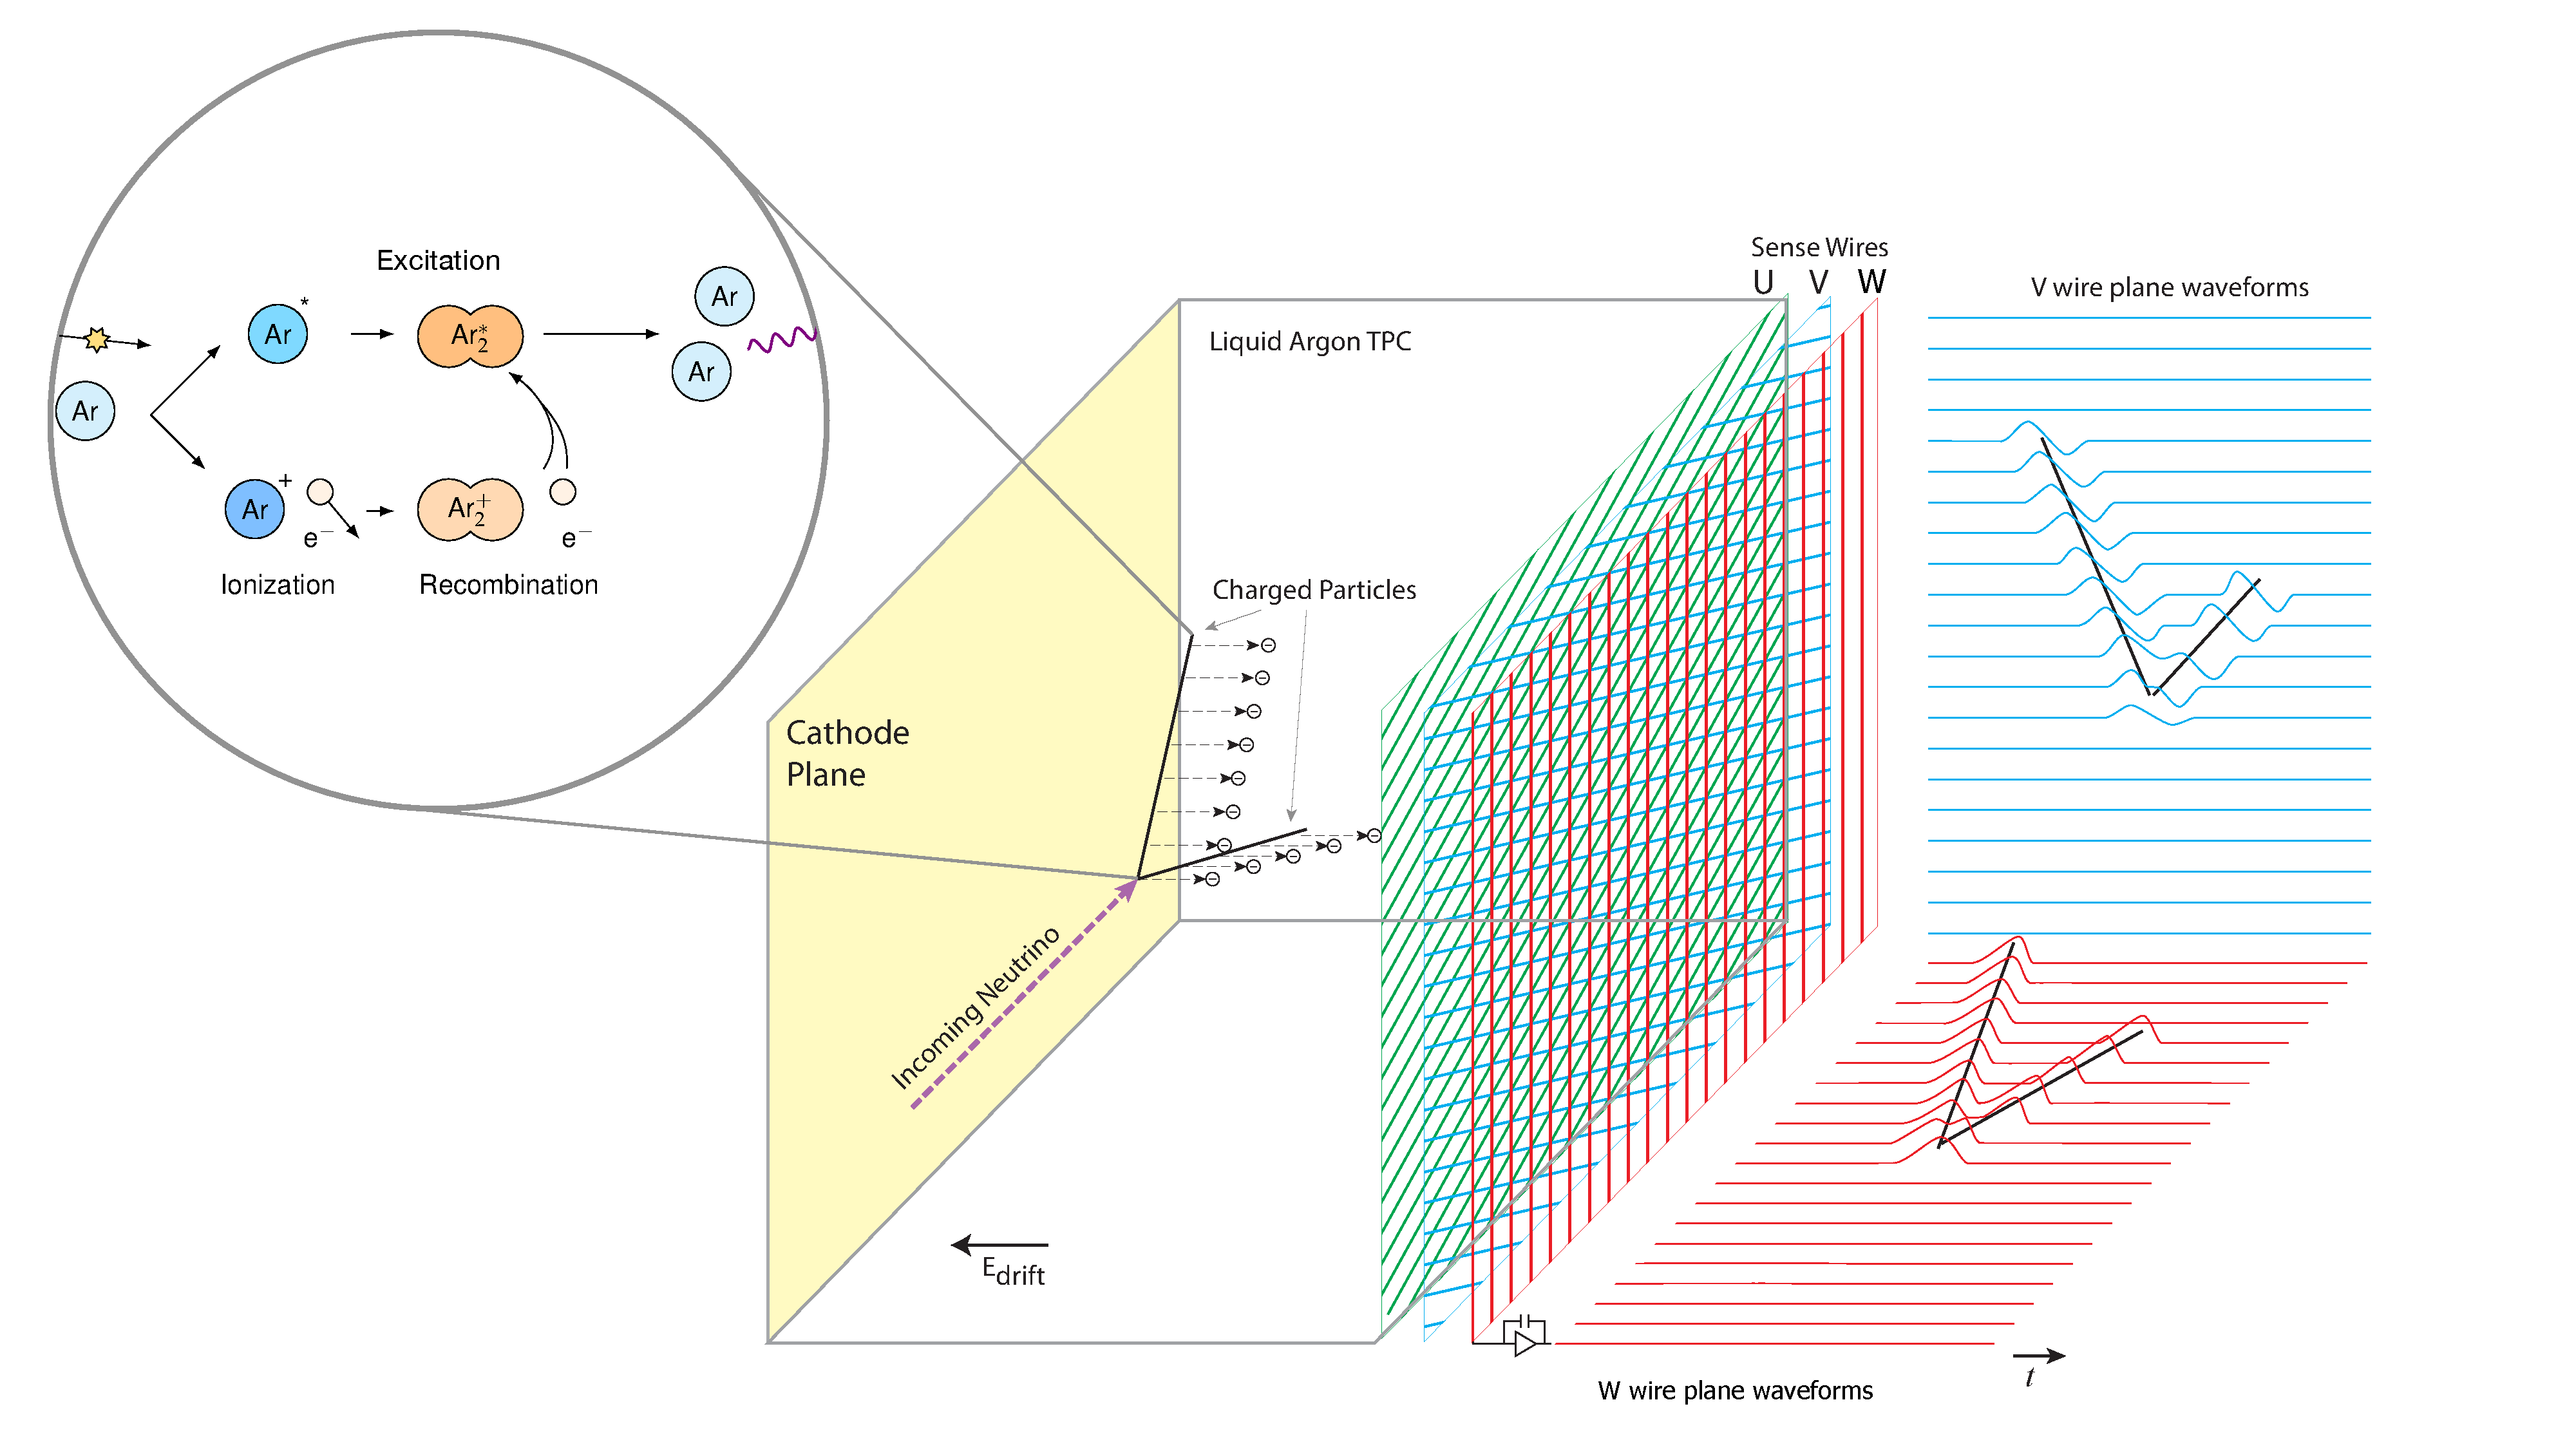
\includegraphics[width=\linewidth, trim={0 0 1.5cm 0}]{thesis/6_figures/detector/TPC_argon.pdf}
    \caption[LArTPC illustration]{Illustration of the working principle of a LArTPC detector. Once neutrinos undergo weak interaction, they ionise the material, producing a large quantity of free electrons that are drifted towards the wireplanes. }
    \label{fig:TPC}
\end{figure}

The first TPCs were built primarily for high energy physics (HEP) applications, and many are still in use for major experiments, such as the ALICE tracker \cite{Lippmann:2014lay}. Carlo Rubbia proposed using liquid argon (LAr) as an interaction target for a TPC, thereby inventing the LArTPC concept for neutrino detection \cite{rubbiaLiquidArgonTime1977}. Liquid argon is an attractive material for particle detection, especially for neutrino physics, given its physical properties \begin{enumerate}
    \item LAr has a high density at \SI{1.39}{\gram\per\centi\meter\cubed} and a high atomic mass, which, combined with the small cross-section of $\PGn$-Ar interaction, allows for more probable detection than most gases.
    \item Being argon a noble gas, it does not attach free electrons, allowing for a longer drift lifetime.
    \item It has high electron mobility, $\mu\simeq \SI{320}{\centi\metre\squared\per\volt\per\second}$ for $E\simeq\SI{0.5}{\kilo\volt\per\centi\metre}$ and $T=\SI{87}{\kelvin}$, allowing for fast drift velocity $v=\mu E \simeq \SI{1.6}{\metre\per\milli\second}$.
    \item The LAr radiation length $X_0\simeq\SI{14}{\centi\metre}$ allows mm-scale calorimetry sampling of neutrino events while having a precise discrimination between electron- and photo-induced electromagnetic showers. Photons produced at the primary vertex usually show a greater conversion gap between the interaction and the starting points of the EM shower; additionally, photo-induced electromagnetic showers display an ionisation pattern in the first centimetres of the shower development compatible with two minimum ionising particles (MIP), whereas electron-induced showers show a pattern compatible with a single MIP.
    \item Ar is both easy and cheap to obtain. In Earth's atmosphere, it is the third most abundant gas, and can be liquified using nitrogen: this allows for great scalability required to use it for large-scale detectors.
    \item LAr boiling temperature of \SI{87.3}{\kelvin} causes most organic impurities to be frozen out to very low levels. This increases the drift electron lifetime. 
\end{enumerate}

Inside a LArTPC, once the neutrino undergoes weak interaction, it produces secondary charged ionising particles. These ionise LAr nuclei, creating $\mathrm{Ar^+},\ \Pem$ ionisation pairs and producing scintillation light. Roughly \SI{42}{\kilo e} are produced for each MeV of deposited energy\footnote{This number is dependent on the electric field strength inside the detector. This value is the reference with a nominal electric field of $\sim \SI{500}{\volt\per\centi\meter}$.}, which are then drifted by means of an electric field toward the anode plane assembly (APA). At the anode three planes of wires are placed in sequence, referred to as induction-1 (I-1), induction-2 (I-2) and collection (C) planes --- \autoref{fig:TPC} shows the common convention, which is to call the three planes U (I-1), V (I-2) and W (C). The planes are properly voltage biased to achieve a nearly perfect transparency of the first two wire planes (I-1 and I-2) with respect to the drift electrons, enabling them to induce a charge on the first two planes and only be collected by the third plane. Given a nominal electric field inside the detector $E$, a good ``transparency'' of the successive wire planes to the drifting electrons is obtained by requiring that $E_2\geq F\times E_1$, and $E_1 \geq F \times E$ --- where $E_1$ and $E_2$ are respectively the field values in the I-1 to I-2 gap and I-2 to C gap --- with the scaling factor $F\in(1.2, 1.5)$.

The three planes of wires have their wires orientated at different angles to be able to  collect different ``projections'' of the same interaction happening inside the detector. Using this information, it is possible, in the reconstruction stage, to obtain a $\mathcal O(\si{mm^2})$-scale $(y,z)$ image of the interaction. The third $x$ coordinate is recovered using the timing information. In fact, when charged particles cross LAr, aside from creating ionisation pairs, they produce scintillation light, which constitutes a prompt signal used to assign the $t_0$ information. This way, the missing coordinate is reconstructed by comparing the time at which the electron is recorded on the wire with the prompt scintillation reference time $t_0$, and knowing the drift velocity of ionisation electrons inside LAr, $x = v_\mathrm{d}\times (t - t_0)$. 

Contributing to the formation of scintillation light within LAr are two processes, pictured in the inset of \autoref{fig:TPC} \begin{itemize}
    \item excitation of Ar followed by the formation of the excimer state $\mathrm{Ar_2^*}$, which decay with the production of scintillation photons, \begin{equation}
        \mathrm{Ar^* + Ar} \to \mathrm{Ar_2^*} \to \mathrm{2Ar}+\PGg;
    \end{equation}
    \item recombination of ionized argon atoms with a free electron, especially frequent with clouds of $\Pem$ around ionized $\mathrm{Ar^+}$ nuclei, \begin{equation}
        \mathrm{Ar^++Ar} \to \mathrm{Ar_2^+}\Pem \to \mathrm{Ar_2^*} \to \mathrm{2Ar}+\PGg;
    \end{equation}
\end{itemize}

These two processes combined produce \num{20000} monochromatic vacuum ultraviolet (VUV) photons per MeV of deposited energy, with a wavelength of $\lambda = \SI{128}{\nano\metre}$. This light presents two components, one so-called ``fast'', with a characteristic time $\tau\sim\SI{6}{\nano\second}$, and one ``slow'', $\tau\sim\SI{1.5}{\micro\second}$ components. Scintillation light is crucial, as already mentioned, for precise determination of the global timing required to reconstruct the missing coordinate in the 3-dimensional interaction from the 2-dimensional ``views''. Additionally, as I will briefly discuss later on, scintillation light is core for double-checking the $(y,z)$ positioning of the interaction, providing the so-called ``light barycenter''. 

It should be noted, however, that aside from all the mentioned great properties, there are some drawbacks to the use of LAr for particle detection. First and foremost, a complete understanding of the $\PGn$-Ar interaction has not been reached yet, so there are great systematic uncertainties related to the parametrisation of the interaction cross-section. Secondly, in order to keep argon in its liquid phase and minimise the organic impurities, a great effort is required for the design of the cryogenic infrastructure. 

Whilst this latter problem is intrinsic to the LArTPC design and requires ad hoc designs and implementations of the cryogenic infrastructure to be optimised, the former problem is addressed in the SBN programme by using two functionally identical LArTPC detectors, which allows the cancellation of many systematic uncertainties when performing a joint oscillation analysis. 

Finally, even though LAr was chosen for its large electron mobility, LArTPCs are intrinsically slow detectors, with drift times in the order of milliseconds. Hence, detectors operating at shallow depth, much like the two LArTPCs in the SBN programme, during the readout time window record significant cosmic activity. This reason led both the SBND and ICARUS collaborations to design the detectors to include an external cosmic ray tagger detector system (CRT) with nearly complete $4\pi$ coverage to veto most of the cosmic activity. 

\section{The SBN near detector: SBND} 

The Short Baseline Near Detector, SBND, is the near detector of the SBN programme at Fermilab. Positioned at a distance of \SI{110}{\metre} from the proton-beryllium interaction target, with a total mass of \SI{112}{\tonne} of LAr, SBND will provide a precise flux measurement of unoscillated neutrinos for the far detector, ICARUS. SBND as a ``flux monitor'' will allow a great reduction of the impact of systematic uncertainties related to the interaction of neutrinos in argon and the event reconstruction inside a LArTPC. After nearly a decade of design, construction, and installation, SBND began operation in July 2024 and started collecting stable BNB data in December 2024 with an unprecedented rate of $\sim\num{7000}$ neutrino events per day \cite{SBND:2025lha}. 

As for the ICARUS experiment, the physics goals of the SBND collaboration extend beyond the search for eV-scale sterile neutrinos; making use of its huge statistics, due to its proximity to the beam source point, SBND will allow for extremely precise $\PGn$-Ar interaction cross-section measurements in both the sub-GeV and GeV energy ranges. Additionally, the proximity to the neutrino source point allows the detector to cover both the on-axis as well as the off-axis phase space for BNB, expanding its capabilities to BSM physics studies like what is possible using NuMI for the ICARUS detector. 

SBND's LarTPC consist of a single module, with dimensions of $\qtyproduct[product-units = power]{5x4x4}{\meter}$, holding a total of \SI{112}{\tonne} of LAr. The structure contains two TPCs sharing two common cathode plane assemblies (CPAs) at the centre, parallel to the beam direction, and four anode plane assemblies (APAs) at the other two ends. The maximum drift length for the SBND detector is \SI{2}{\meter} which, for the nominal electric field of \SI{500}{\volt\per\cm}, leads to a maximum drift time of \SI{1.3}{\ms}. Each APA holds three planes of wires spaced \SI{3}{\mm} apart from each other, each hosting \num{2816} wires orientated at \SI{+-60}{\degree} (I-1/U and I-2/V, respectively) and \SI{0}{\degree} with respect to the vertical $y$ axis. 

\section{The ICARUS-T600 detector} 

\begin{sidewaysfigure}
    \centering
    \begin{tikzpicture}
        \node at (0,0) {\includegraphics[width=\linewidth]{detector/SBN-FD_composite}};

        \draw[-*, white] (-1,2.5) node [left, white, fill=Gray!15!black] {TPC electronics} -- (0.5,2.25);
        \draw[-*, white] (-9,.5) node [right, white, fill=BrickRed] {Warm vessel} -- (-7.25,-1.5);
        \draw[-*, white] (4,2) node [right, white, fill=Plum!50!black] {Cryogenics} -- (3.25,3.5);
        \draw[-*, white] (7,-0.5) node [below, white, fill=Gray!15!black] {Top-CRT} -- (6.5,4);
        \draw[-*, white] (6,-1.75) node [right, white, fill=Gray!15!black] {Side-CRT} -- (5,-1);
        \draw[-*, white] (6,-3) node [above, white, fill=Gray!15!black] {Bottom-CRT} -- (3.5,-3.75);

        \draw[-*, white] (0,-4.5) node [below, white, fill=Gray!25!black] {East T300 cryostat} -- (-1,-3.5);
        \draw[-*, white] (-4.5,-4.5) node [left, white] {
            \begin{minipage}{4cm}
                \raggedleft
                TPC wireplanes + PMTs
            \end{minipage}} -- (-2.5,-2.5);

        \draw[-Latex, white] (-7,-3.5) -- (-7, -2.5) node[above] {$y$};
        \draw[-Latex, white] (-7,-3.5) -- (-6, -3.2) node[right] {$z$ (beam)};
        \draw[-Latex, white] (-7,-3.5) -- (-7.5, -3.35) node[left] {(drift) $x$};

        \draw[-*, black] (-4.5,5) node [left, black] {\SI{3}{m} concrete overburden} -- (-3,4.5);

        % \draw[step=1.0,white,thin] (-10,-5.5) grid (10,5.5);
        % \foreach \i in {-10,...,10} {
        %     \node [below] at (\i,-5.5) {$\i$};
        % }
        % \foreach \i in {-5,...,5} {
        %     \node [left] at (-10,\i) {$\i$};
        % }

        
    \end{tikzpicture}
    \caption[ICARUS detector illustration]{Illustration of the ICARUS T600 detector at Fermilab. Surrounding the warm vessel is the $4\pi$ coverage CRT. Above the warm vessel, the TPC readout warm electronics are placed, alongside the proximity cryogenics. Inside the warm vessel two identical (east and west) T300 modules are hosted, each containing two TPCs sharing a common cathode at the centre and two anode plane assemblies, one on each side.}
    \label{fig:ICARUS_scheme}
\end{sidewaysfigure}

\subsection{The ICARUS subsystems} 

\paragraph{TPC} 

\begin{figure}
    \centering
    \subfloat[]{\includegraphics[height=5.5cm]{thesis/6_figures/detector/TPC_wires_texts.pdf}}
    \hspace{1em}
    \subfloat[]{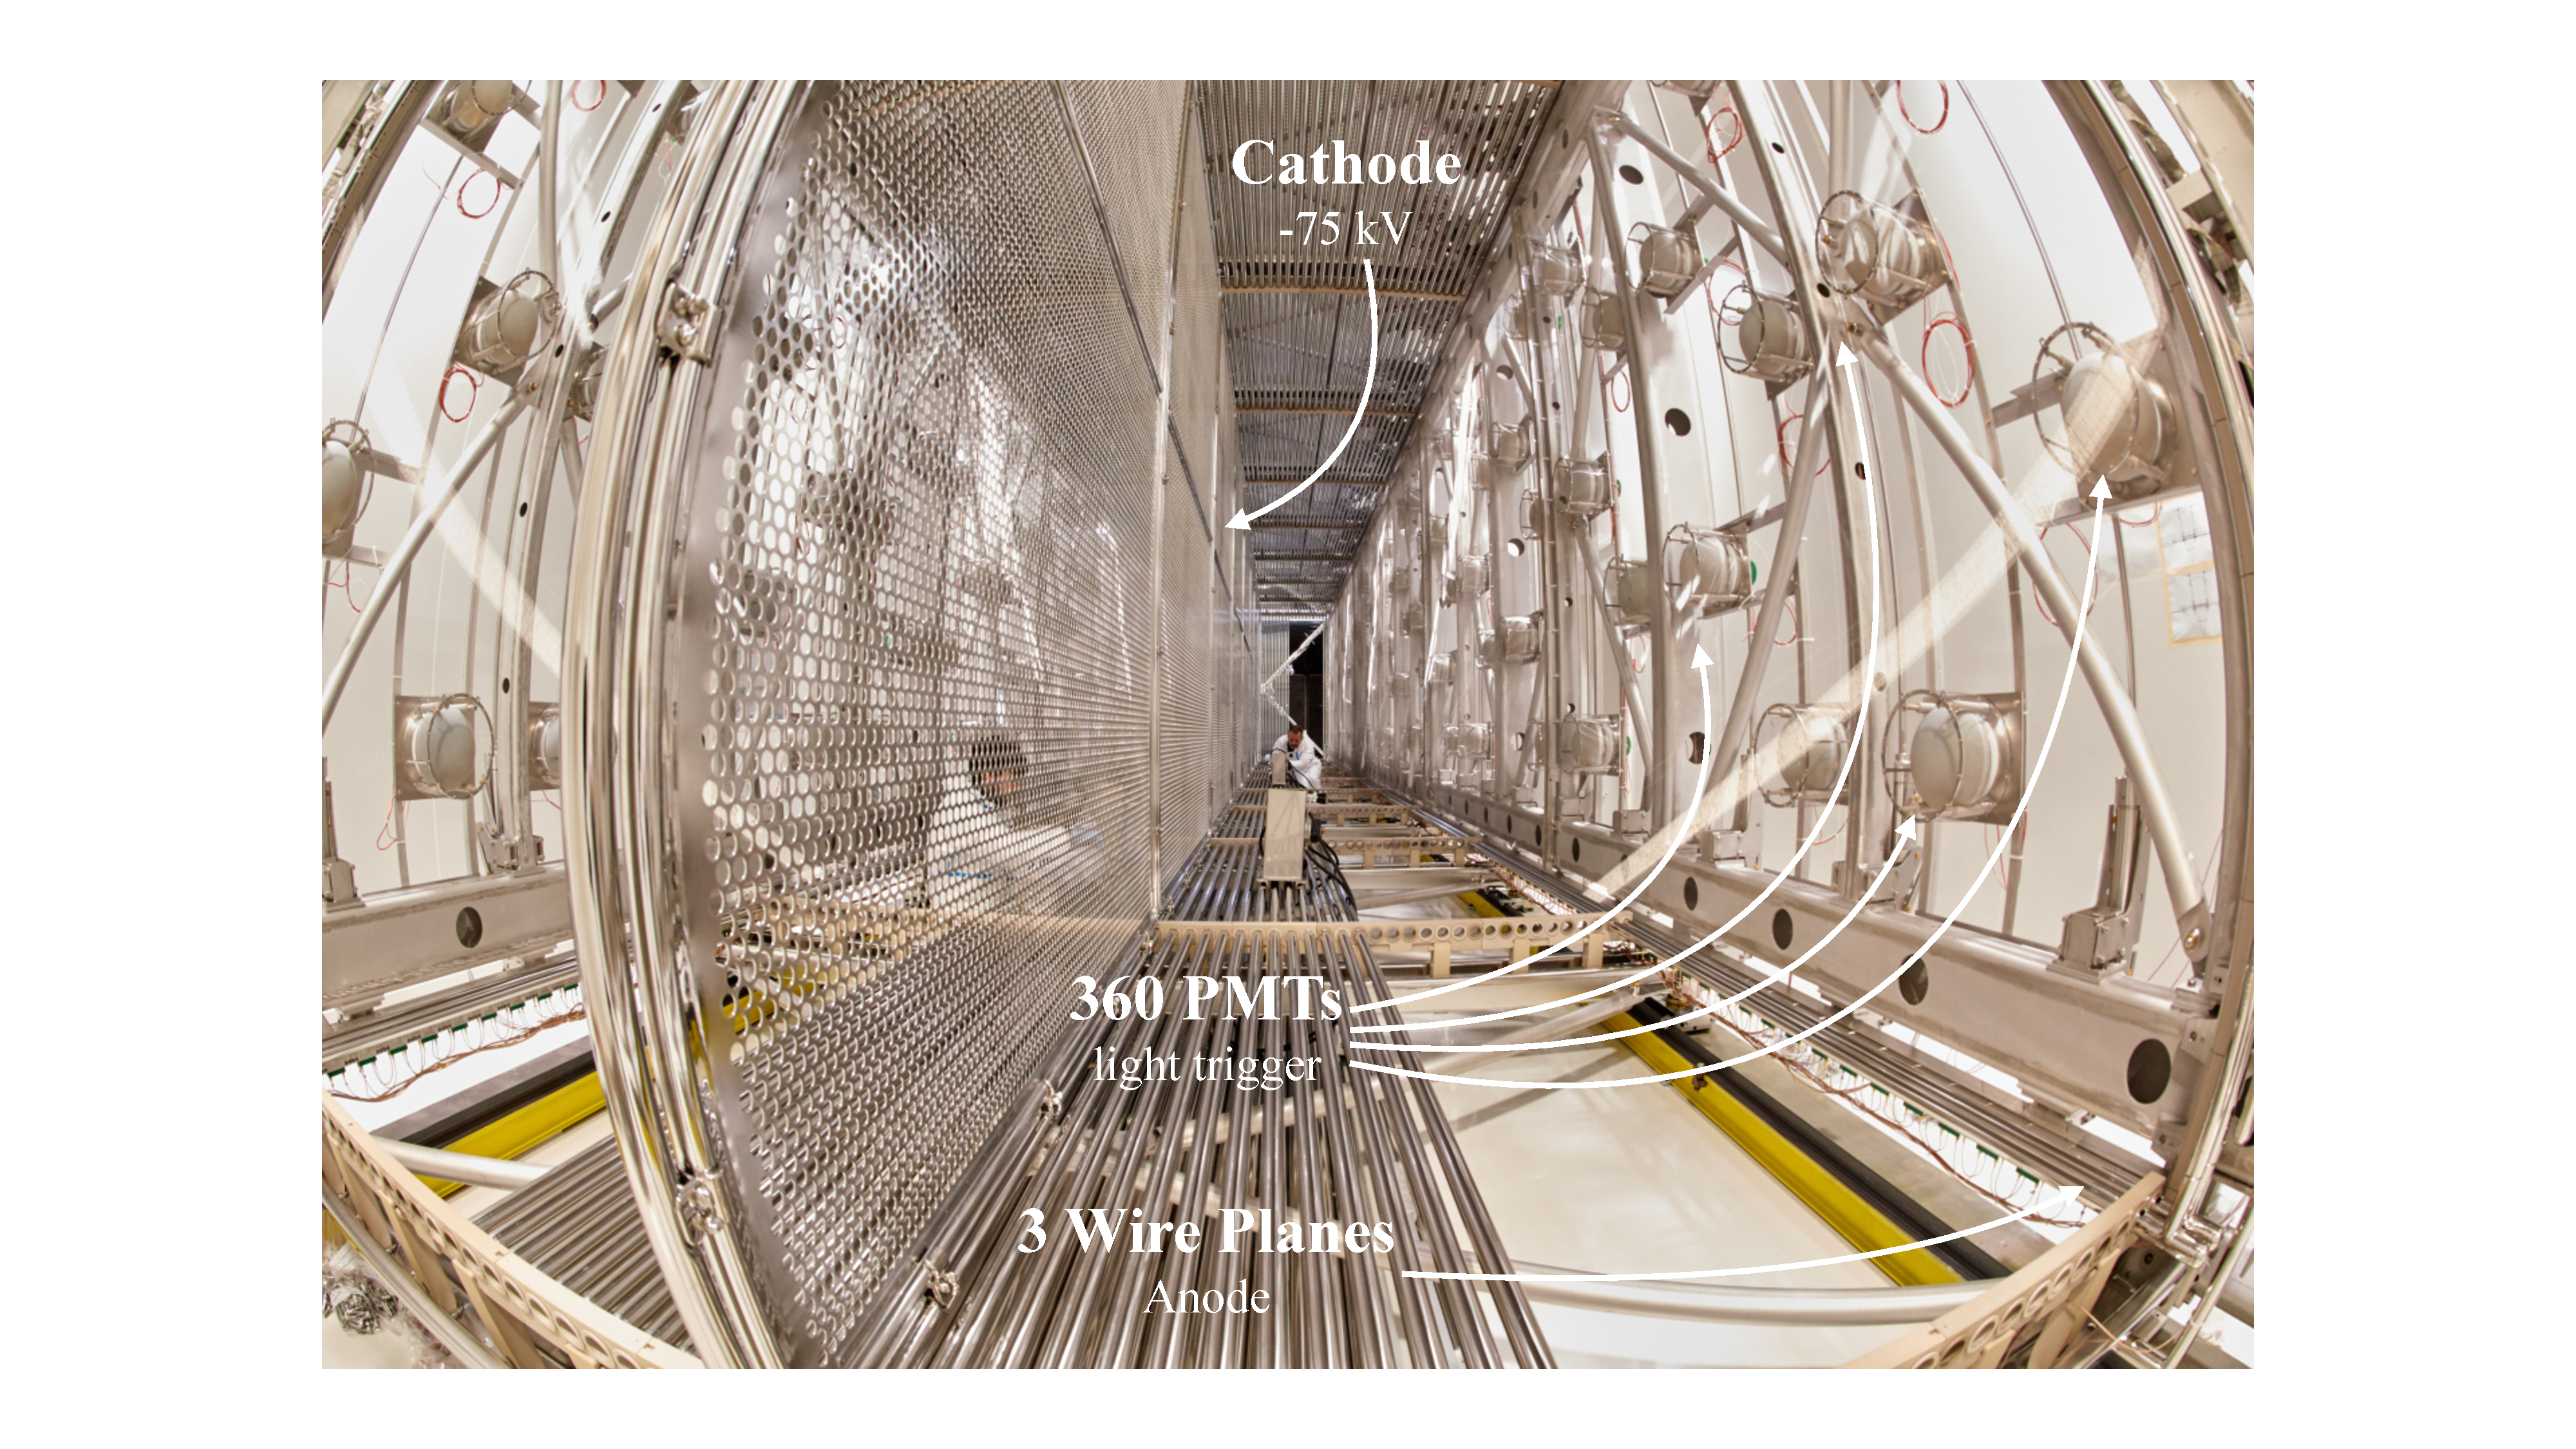
\includegraphics[height=5.5cm, trim={8cm 2cm 8cm 2cm}, clip]{thesis/6_figures/detector/TPC_inner.pdf}}
    \caption[ICARUS TPC wires and field cage]{}
    \label{fig:ICARUS_photo}
\end{figure}

\paragraph{Light collection system} 

\paragraph{Cosmic ray tagger} 


% Firstly proposed by Nobel laureate Carlo Rubbia \cite{Rubbia:1977zz}, the concept of Liquid Argon Time Projection Chambers (LArTPCs for short) was implemented in the Gran Sasso National Laboratories (LNGS) near L'Aquila (Italy) in the ICARUS (Imaging Cosmic And Rare Underground Signals) detector \cite{Bettini:1991fh, Cennini:1994pk, Cennini:1995tt, ICARUS:1995nrd}, which collected data between 2006 and 2011 \cite{Rubbia:2011ft}, alongside the OPERA, LVD and BOREXINO detectors from the CERN Neutrinos to Gran Sasso (CNGS) neutrino beam \cite{Kodama:2004db}. The main detectors for this project were the OPERA and ICARUS experiments, and were therefore called respectively CNGS1 and CNGS2.

% Today, the ICARUS T600 detector is one of the longest running LArTPC in existence. 

% After the results of the CNGS analysis were published the ICARUS detector moved in 2018 from LNGS, to the CERN facility, where it underwent a series of upgrades, both for electronics and in the liquid Argon purification system; serious upgrades were also performed on the exterior of the experiment where a cosmic ray tagger module was added; in 2020 the detector arrived to its current location in the SBN facility at Fermilab, where it has been detecting neutrinos since: mainly $\PGnGm$ and some $\PGne$s, from the Booster Neutrino Beam (BNB, on axis with the $z$ direction of the detector frame of reference) and from the Neutrino Main Injector (NuMI). 

% At the Short Baseline Neutrino (SBN) facility, the ICARUS experiment started its data run taking period in 2022 and has since ran thrice \cite{ICARUS:2023gpo}, with the latest data expected to be ready for the end of 2024 for the official analysis. Its younger brother, the SBND (Short Baseline Near Detector) experiment, finished the cryostat commissioning with some delays in 2023 and is now completing the commissioning of the cosmic ray tagger (CRT) modules, with the analysis on veto efficiency for the top CRT modules ongoing. 

% Joint efforts of the SBND and ICARUS detectors in the SBN collaboration will provide a highly efficient identification of neutrino interactions, strongly mitigating the possible sources of background and reducing the impact of systematics. 

% The combination of two nearly identical detectors allows for the measurement of neutrino oscillations over the distance in between the experiments, comparing the $\nu$s flux at \SI{110}{\meter} (SBND) and at \SI{600}{\meter} (ICARUS). 

% A third and a fourth experiment were also active in the BNB baseline, MiniBooNE (\mboone) and MicroBooNE (\uboone). The former completed its data taking period in 2018, and the latter was active between 2015 and 2021. Those two experiments provided strong ($\sim5\sigma$) evidence of event excess \cite{MiniBooNE:2018esg} in respect to what was expected (see figure \ref{fig:miniboone_results}). The main goal of the SBN collaboration is therefore to test this anomaly using data from BNB neutrinos. 

% In addition to this anomaly, ICARUS will also test the oscillation signal reported by the Neutrino-4 collaboration, hinting towards $\Delta m^2 \simeq \SI{7.26}{\electronvolt\squared}$ and $\sin^22\theta = 0.38$ ($3.5\sigma$ CL), both in $\PGne$ and $\PGnGm$ channels from BNB and NuMI.